\subsection{Preprocessing techniques}
In this section, we have implemented the preprocessing techniques described above to different levels of attack, to be more specific, the $\epsilon$ in FGSM attack and a higher $\epsilon$ represents a higher level of attack. Results of accuracy versus attack are provided below, with various values of parameters in different techniques.

\subsubsection{Bit-Depth Reduction}
The dataset used here is MNIST 28 by 28 images set with original channel 8 bits. The systems we use here are both the fully pretrained model with 98.1\% accuracy, and our manually trained model with 94.75\% accuracy in the original test set. We apply bit-depth reduction technique to the input images just before feeding our system, adding a preprocessing layer. 
\begin{figure}[h!]
	\centering
	\begin{subfigure}{.4\textwidth}
		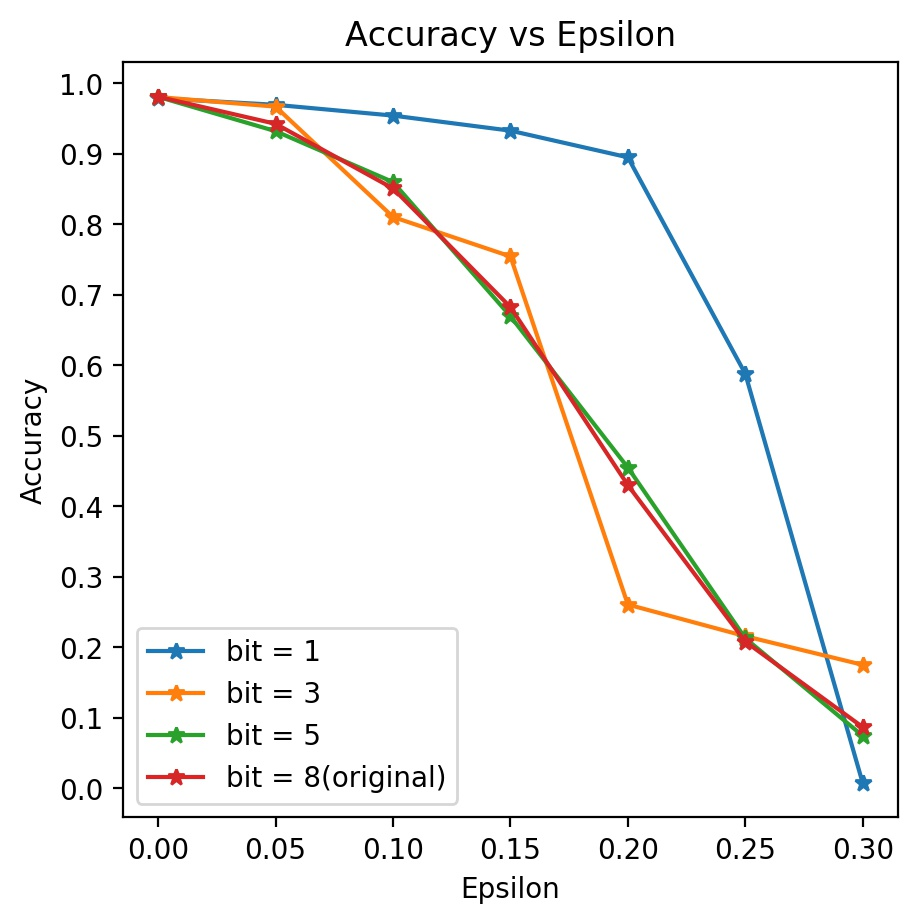
\includegraphics[width=\textwidth]{pretrained_Accuracy_vs_Epsilon_db.jpg}
		\caption{pretrained model}
		\label{fig: bit-depth reduction pre}
	\end{subfigure}
	\begin{subfigure}{.4\textwidth}
		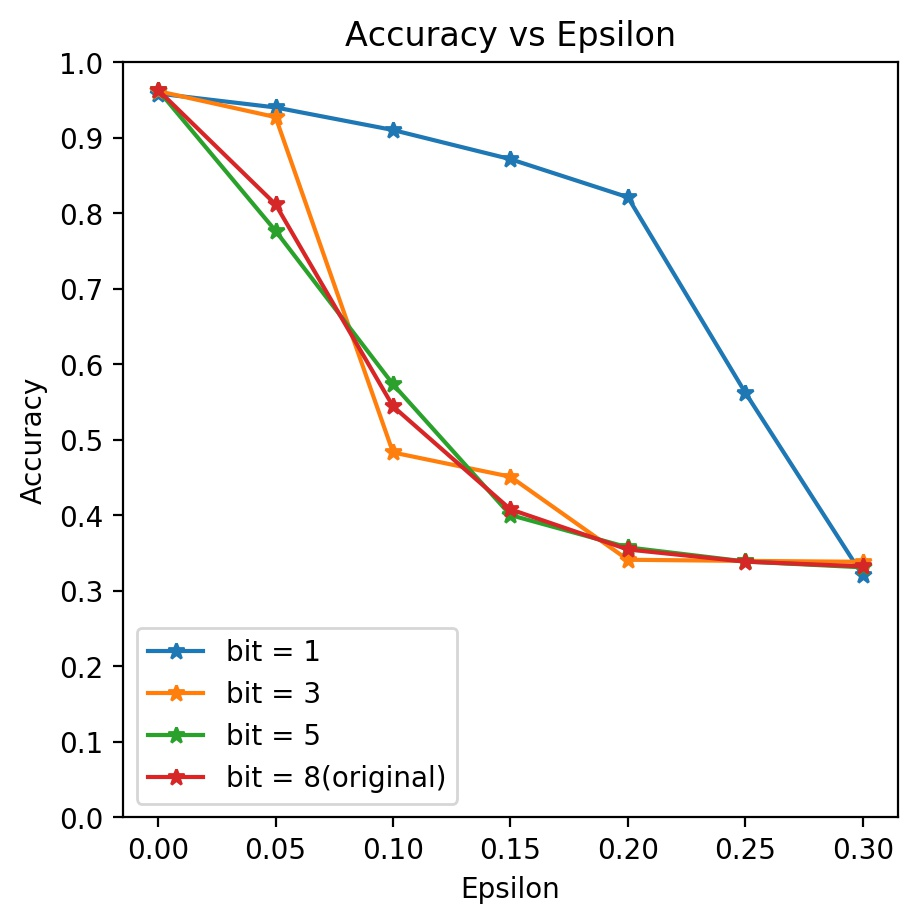
\includegraphics[width=\textwidth]{Accuracy_vs_Epsilon_db.jpg}
		\caption{Our model}
		\label{fig: bit-depth reduction us}
	\end{subfigure}
	\caption{Accuracy for different levels of noise we choose}
\end{figure}

We can see in both cases, bit-one reduction performs the best except we increase the adversarial level $\epsilon$ to 0.3 for the pretrained model, where its accuracy is less than 0.1, worse than random guess. Also, in both cases, as we decrease the bit for each channel, the relative accuracy increases, with some fluctuation. But it is shown that bit-depth reduction can introduct human-noticeable loss in more complex images for bits less than 4 \cite{DBLP:journals/corr/XuEQ17}. One interesting we notice here is that, although our manually trained model does not perform as well as the pretrained model in the original testing set, it is shown to be more robust to the adversarial attack, in the sense that its accuracy reduce slower for higher level adversarial attack. But in both cases, the accuracy is still lower than what we expect.  


\subsubsection{Total Variation Minimisation} 
We use the same dataset and models here, and apply total variation minimisation technique with different weights which represent the portion expected portion to be replaced, $p = 2$ for $l_p$ norm, and the algorithm of Rudin, Fatemi and Osher that was proposed by Chambolle \cite{Chambolle:2004:ATV:964969.964985} for the optimisation. 

\begin{figure}[h!]
	\centering
	\begin{subfigure}{.4\textwidth}
		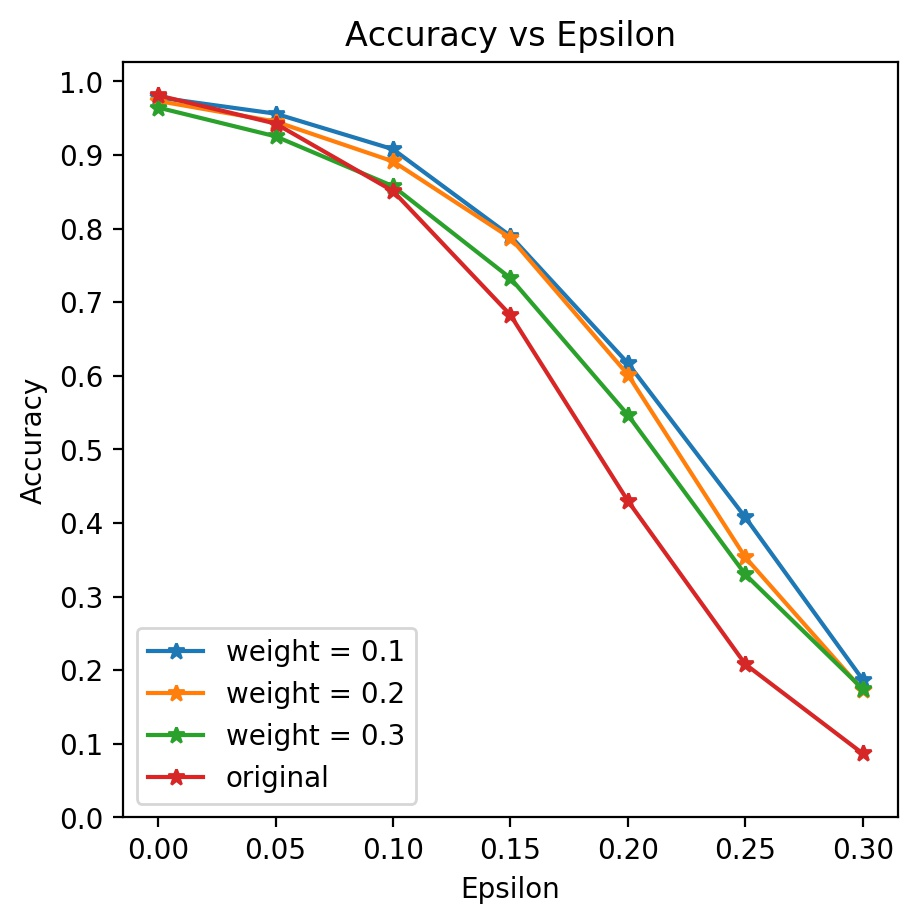
\includegraphics[width=\textwidth]{pretrained_Accuracy_vs_Epsilon_tv.jpg}
		\caption{pretrained model}
		\label{fig: tv pre}
	\end{subfigure}
	\begin{subfigure}{.4\textwidth}
		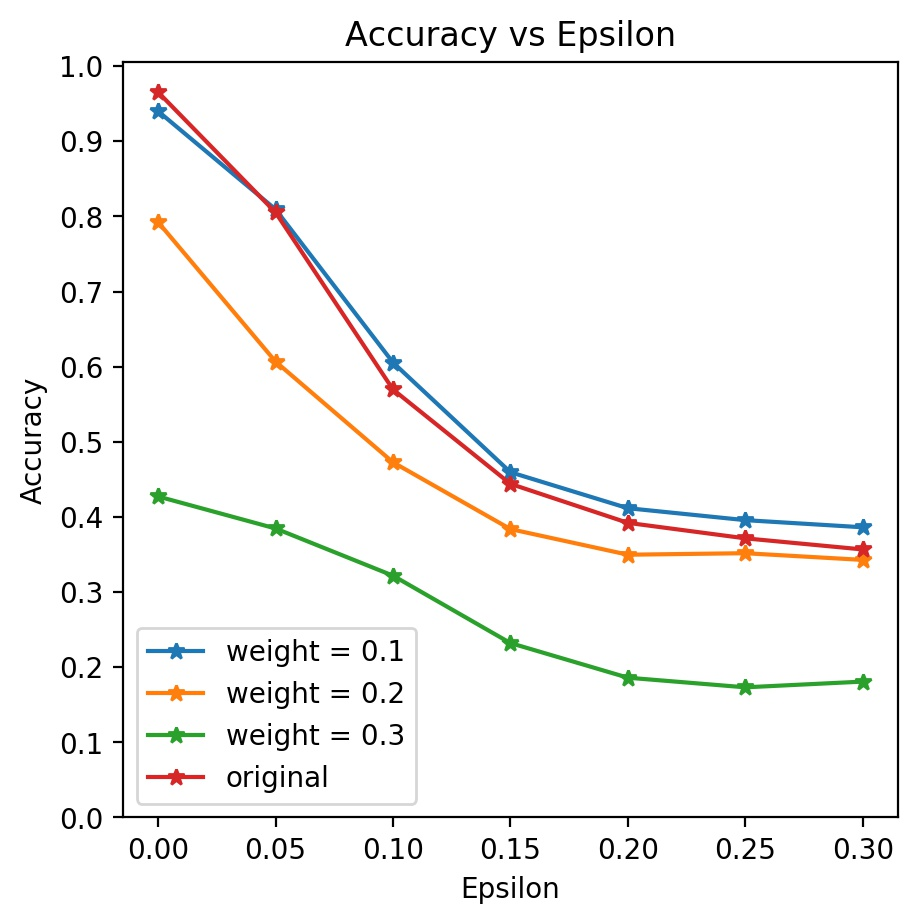
\includegraphics[width=\textwidth]{Accuracy_vs_Epsilon_tv.jpg}
		\caption{Our model}
		\label{fig: tv us}
	\end{subfigure}
	\caption{Accuracy for different levels of noise we choose}
\end{figure}

The results have similar trend to bit-depth reduction for pretrained model, where the accuracy decrease rapidly when we increase the attack level $\epsilon$. But this time, results of all three weights in our pretrained model are significantly better than the original one.  And our manually trained model is also shown to be more robust to higher level of attack, and the case of low accuracy with even no adversarial attack may be because our model is not trained fully. Hence, for total variation minimisation, it help the system defend against attack more efficiently with the requirement that we have trained the model fully. 



\subsubsection{Resolution reduction}

As per our description in methods section, we perform two resizing operations on the MNIST dataset. The original images are 28 by 28 pixels, so we scale test images down to 14 by 14, 20 by 20 or 24 by 24, then rescale back to 28 by 28.  We see from Figure \ref{fig:resolution} that this method does not appear to work since the model trained on the original data (with stochastic gradient descent) seems more robust. It can be seen that the accuracy decreases immensely in the 14 by 14 case, suggesting the scale chosen is too extreme to be able to clearly distinguish the class. When the magnitude of \(\epsilon\) is increased to 0.15, the rescaled samples had accuracy no better than random guessing. The poor accuracy could be due to the fact that the boundaries are blurred when we scale down and back-up again, making those regions more sensitive to perturbations, although further investigations could be carried out on other datasets to confirm this.

\begin{figure}[h!]
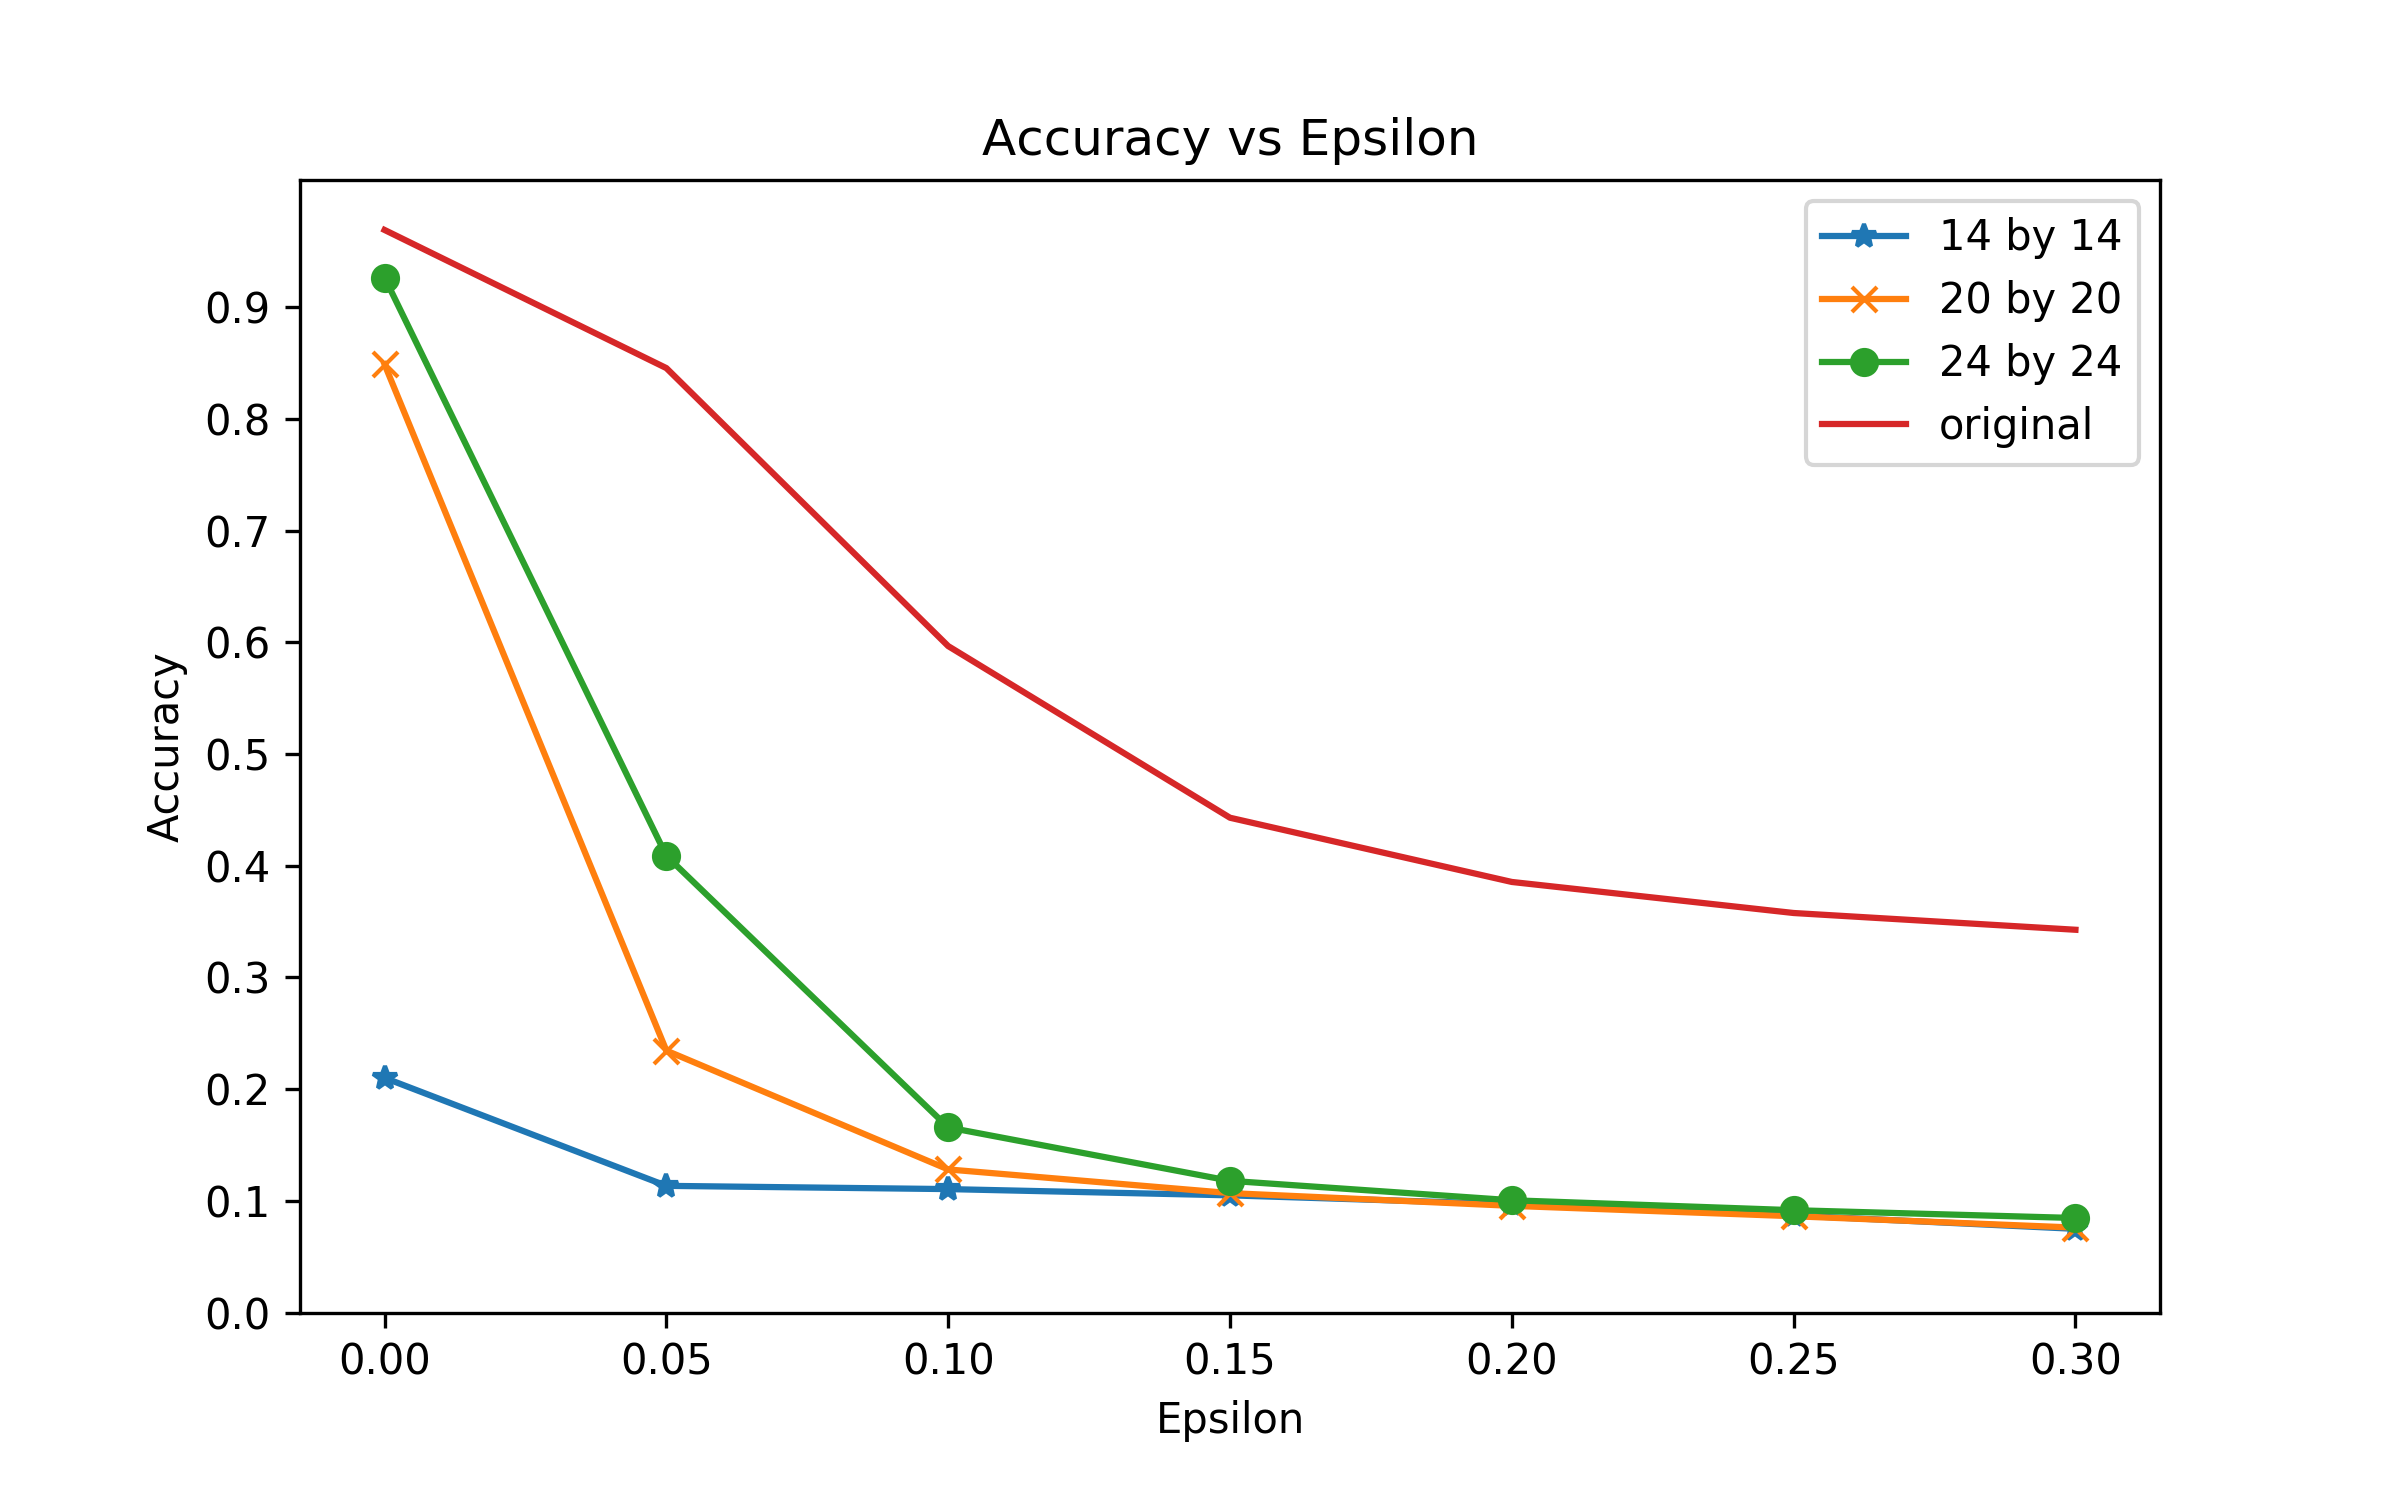
\includegraphics[width=\textwidth]{rescaled_adam}
		\caption{Accuracy in classification under FGSM attacks after a range of rescaling to reduce image resolution.}
		\label{fig:resolution}

\end{figure}

\subsection{Randomised Crop-and-rescale}

We applied 30 randomised crop-and-rescale transformations onto each test subject and then feed all 30 transformed images into the neural network. We record the final classification of the original image as either the mode of the output classes or the class with the highest average sigmoid value across the 30 transformations. The results of such transformations can be seen in Figure \ref{fig:rand}. For lower magnitude of errors using the original test images seem to be better, however the situation is reversed when epsilon increases beyond 0.15. It appears that this method is more robust for perturbations of higher magnitude.

\begin{figure}[h!]
        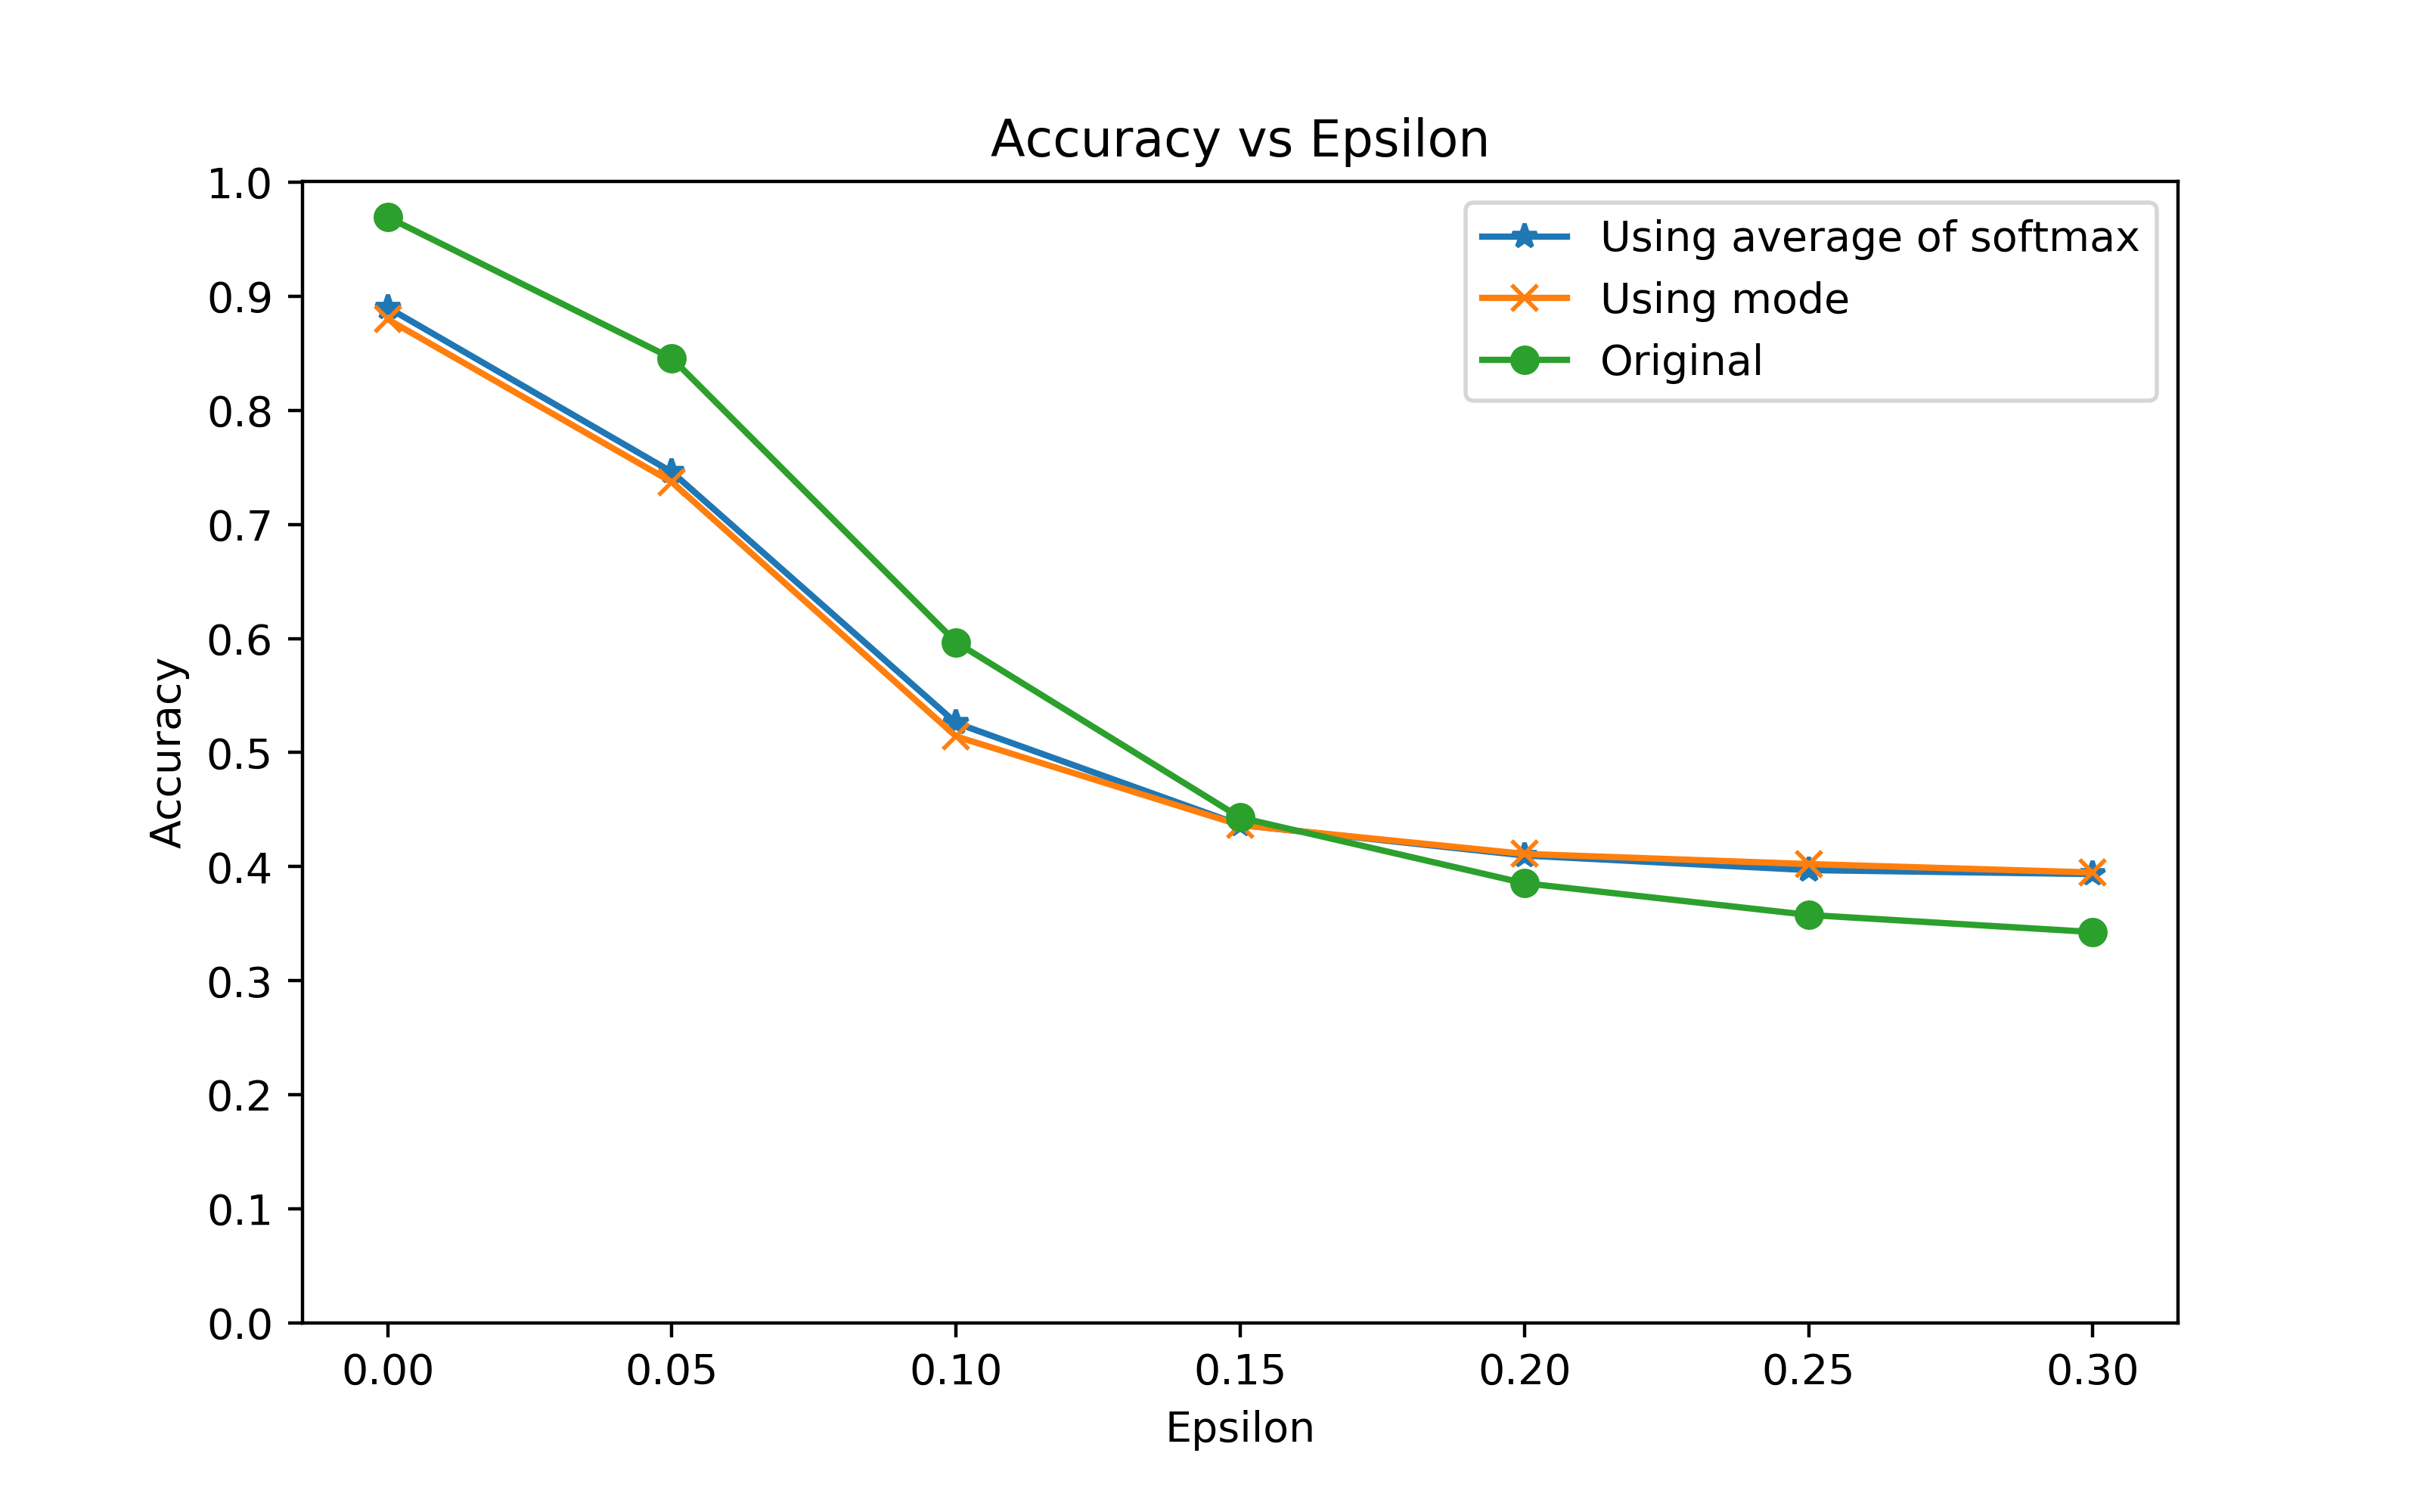
\includegraphics[width=\textwidth]{sgd_random}
		\caption{Accuracy in classification under FGSM attacks using randomised crop-and-rescale transformations}
		\label{fig:rand}
\end{figure}

\subsubsection{Defence GAN}
\begin{figure}[h!]
	\centering
	\begin{subfigure}{.4\textwidth}
		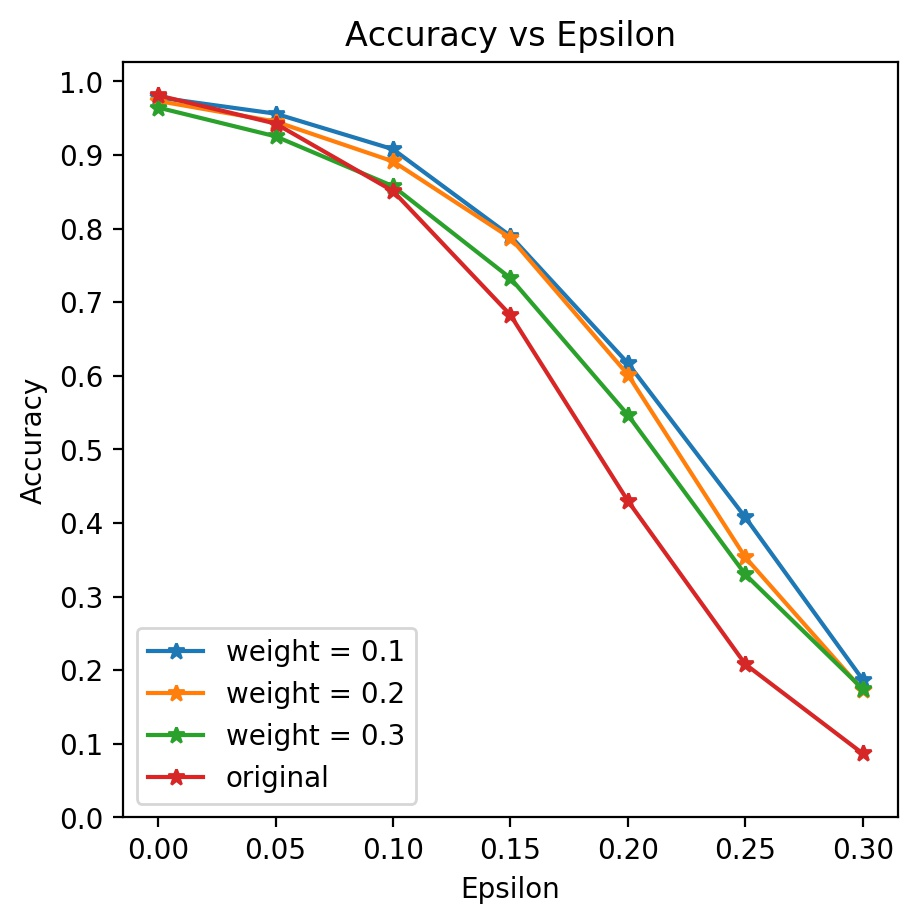
\includegraphics[width=\textwidth]{pretrained_Accuracy_vs_Epsilon_tv.jpg}
		\caption{pretrained model}
		\label{fig: tv pre}
	\end{subfigure}
	
	\caption{Accuracy for different levels of noise we choose}
\end{figure}
